\section{Summary Statistics}
summary statistics are used to summarize a set of observations, in order to 
communicate the largest amount of information as simply as possible. The most 
common types are measurements of location and spread. Below are a collection of
examples of summary statistics.

\begin{itemize}
    \item Frequency
    \item Mode
    \item Percentiles
    \item Mean
    \item Median
    \item Range
    \item Variance
\end{itemize}

\subsection{Frequency and Mode}
The frequency of an attribute value is the percentage of time the value occurs 
in the data set. The mode of an attribute is the most frequent attribute value.
These metrics are often used on categorical data. 

\begin{theo}[Frequency]{theo}
    \label{eq:Frequency}
        \[
            \text{Frequency}(x) = N_x = \text{No of occurences of value x}
        \]
\end{theo}

\begin{theo}[Mode]{theo}
    \label{eq:Mode}
        \[
            \text{Mode}(X) = \underset{x}{\mathrm{arg max} } \text{Frequency}(x)
        \]
\end{theo}

\subsection{Percentile}

\begin{figure}
    \centering
    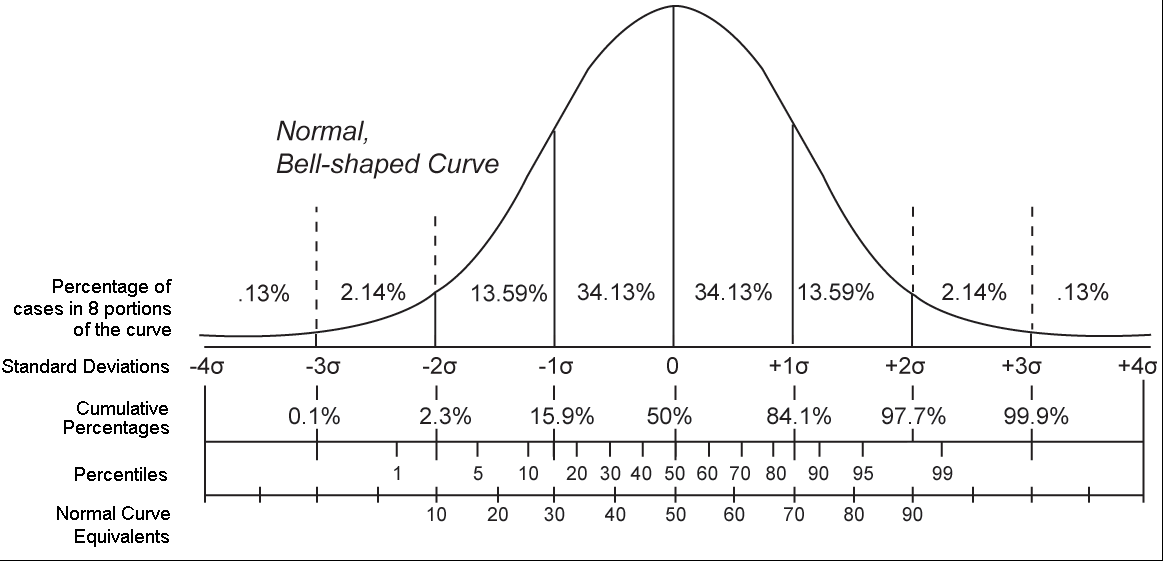
\includegraphics[width=\textwidth]{figures/percentile.PNG}
    \caption{Example of gaussian and it's percentiles}
    \label{fig:percentile}
\end{figure}

In statistics, a percentile is a score below which a given percentage of scores 
in its frequency distribution falls or a score at or below which a given 
percentage falls. See figure \ref{fig:percentile}.

\subsection{Measurements of location}

The most common measurement of location is the mean.

\begin{theo}[Mean]{theo:theo5}
    \label{eq:mean}
        \[
            mean(x) = \bar{x} = \frac{1}{m}\sum_{i=1}^m x_i
        \]
\end{theo}

though the mean is very sensitive to outliers. There are many ways to combat
this sensitivity. One is to use the median.

\begin{theo}[Median]{theo:theo6}
    \label{eq:median}
        \[
            median(x) = 
            \left\{\begin{matrix}
                x_{(r+1)} & \text{if } m=2r+1 \\ 
                \frac{1}{2} \left( x_{(r)} + x_{(r+1)} \right)  & \text{if } m=2r
            \end{matrix}\right.
        \]
\end{theo}

Median is not affected by outliers in the same way since it only cares about the
index of the sorted observations and not the value of the observations itself. 

\subsection{Measurements of Spread}

After we have calculated the location of our distribution, using mean, median or
any other location metric. But this metric only tells us of where the center of
the data lies. The most used metric to describe the spread of data is vatiance:

\begin{theo}[Variance]{theo:theo7}
    \label{eq:variance}
        \[
            variance(x) = s_x^2 = \frac{1}{m-1} \sum_{i=1}^m(x_i-\bar{x})^2
        \]
\end{theo}

Variance as a statistic, like mean, is sensitive to outliers. Therefore there
exists other statistics of spread that are robust.

\begin{theo}[Average Absolute Deviation]{theo:theo8}
    \label{eq:aad}
        \[
            AAD(x) = \frac{1}{m} \sum_{i=1}^m \abs{x_i-\bar{x}}
        \]
\end{theo}

\begin{theo}[Mean Absolute Deviation]{theo:theo9}
    \label{eq:mad}
        \[
            MAD(x) = median \left( \left\{\abs{x_1-\bar{x}} \cdots \abs{x_m-\bar{x}}\right\} \right)
        \]
\end{theo}

\section{Visualisation}
Visualisation is the conversion of data into a visual or tabular format so that 
the characteristics of the data and the relationships among data items or 
attributes can be analyzed or reported. Visualisation allows humans to detect 
general patterns and trends, as well as detect outliers and unusual patterns.
Visualisation therefore is one step of transforming Data into information.

\subsection{Representation}
The representation is the mapping of information to a visual format. 
Data objects, their attributes, and the relationships among data objects are 
translated into graphichal elements such as points, lines, shapes, and colors.

\subsection{Arrangement}
Arrangement is the placement of visual elements within a display. This can make 
a large difference in how easy it is to understand the data.

\subsection{Selection}
Selection is the elimination or the de-emphasis of certain objects and 
attributes. Such selections may involve choosing a subset of attributes, or 
choosing a subset of objects. Only selecting some attributes can be done through 
dimensionality reduction, while selecting some objects can be done through 
stratified sampling. Some things to keep in mind when using data selection is to
contain the diversity of the objects.

\subsection{Visualisation Techniques}
\begin{itemize}
    \item Histogram plot
    \item Box plot
    \item Scatter plot
    \item Matrix plot
    \item Parallel coordinates plot
    \item Star plot
\end{itemize}
